\documentclass[border=10pt]{standalone}

\usepackage{tikz}
\usepackage{tikzsymbols}
\usetikzlibrary{calc,patterns,shapes.geometric}

\def\centerarc[#1](#2)(#3:#4:#5){\draw[#1] ($(#2)+({#5*cos(#3)},{#5*sin(#3)})$) arc (#3:#4:#5);}

\begin{document}
	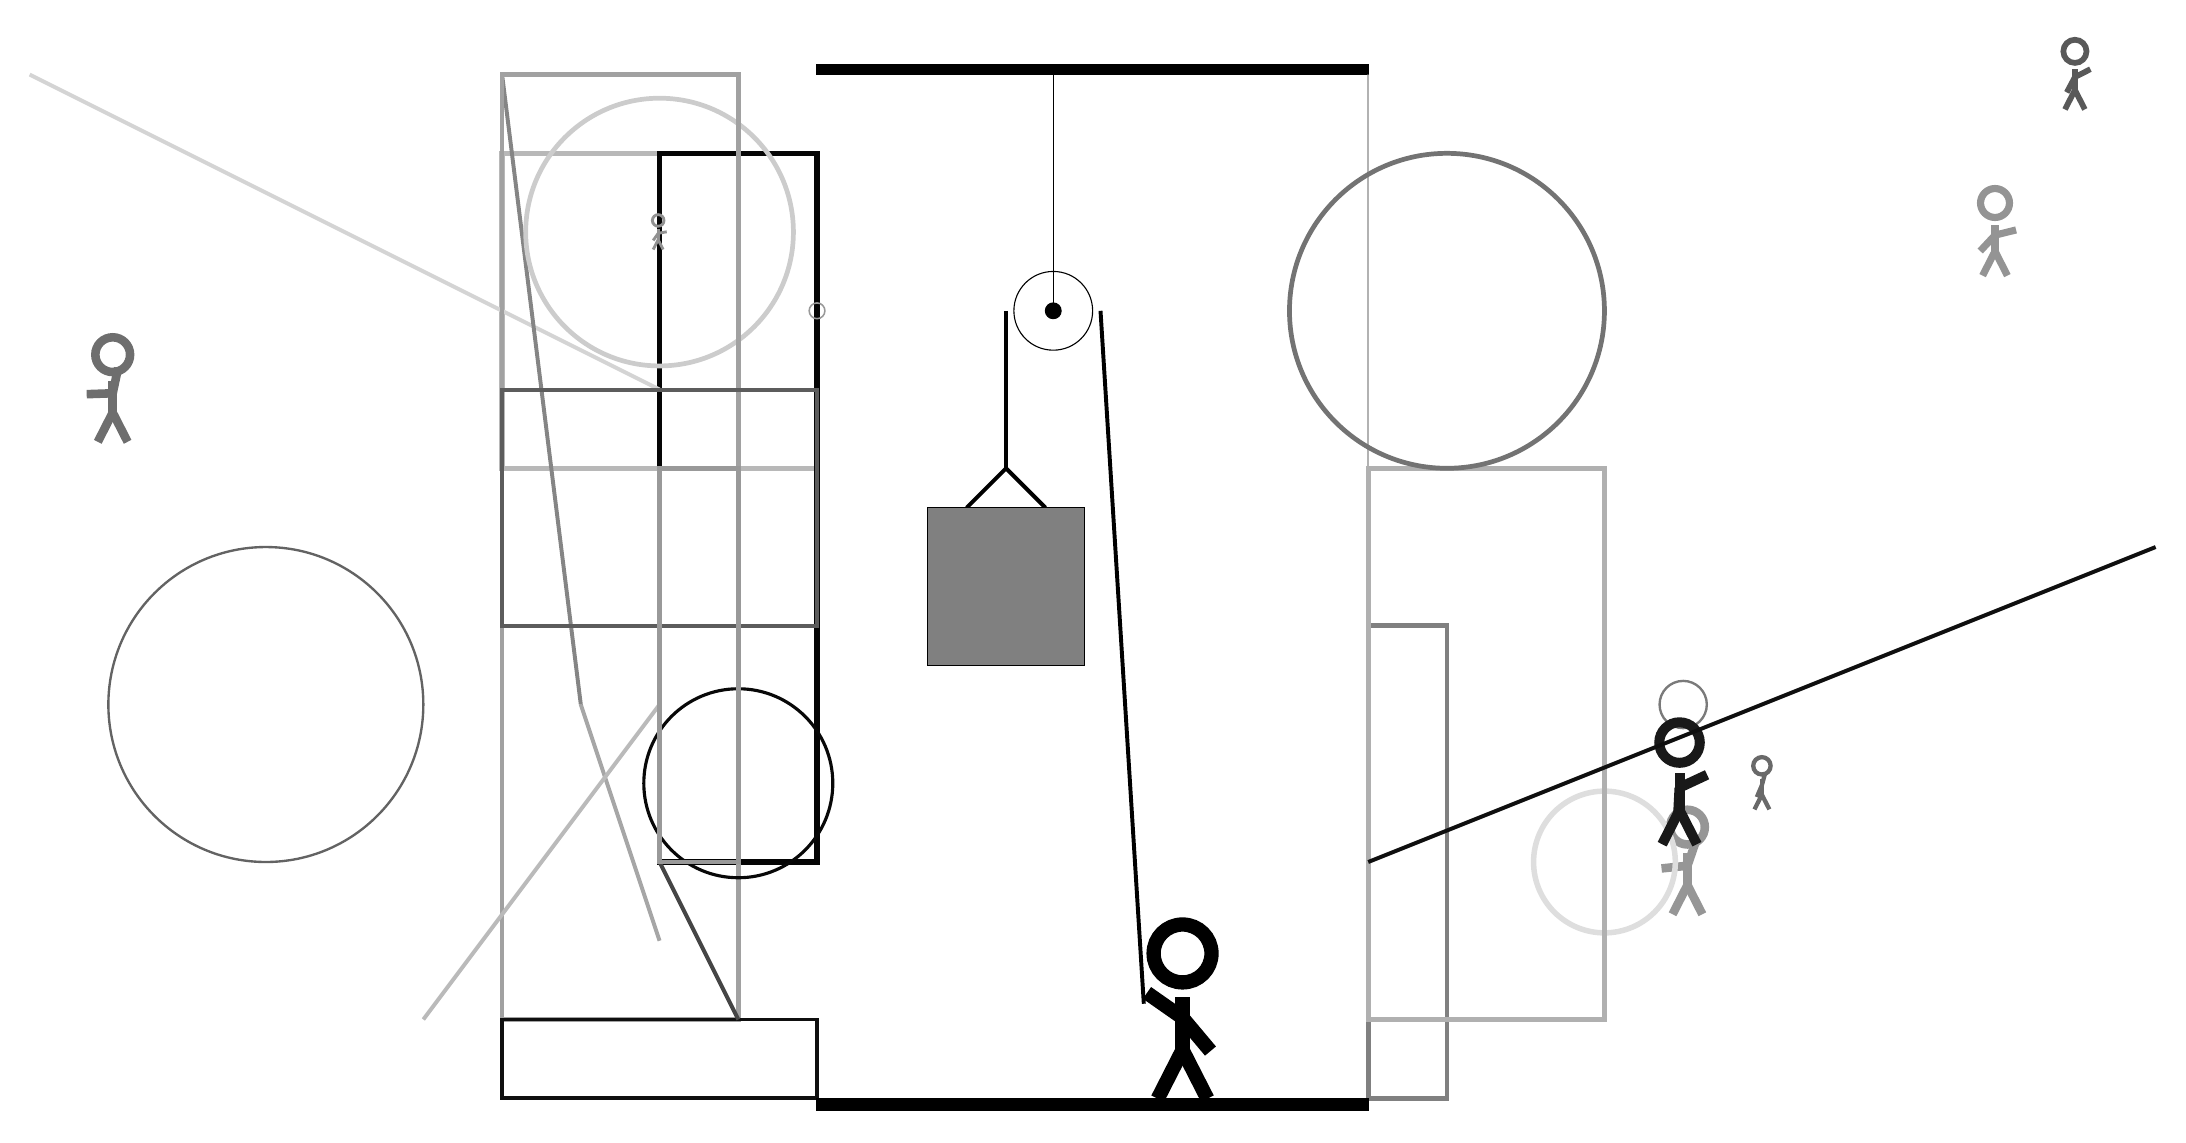
\begin{tikzpicture}
		%%%%% START %%%%%
		
		\draw[fill=black] (-2, 10) rectangle (5, 10.125);
		
		\draw (1, 7) circle (0.5);
		\draw[fill=black] (1, 7) circle (0.1);
		\draw (1, 10) -- (1, 7);
		
		\draw[line width=0.7mm, color=black!28] (-2, 9) rectangle (-6, 5);
		
		\draw [line width=0.3mm, color=black!61](-9, 2) circle (2.0);
		\draw[line width=0.7mm, color=black!98] (-4, 9) rectangle (-2, 0);
		\draw[line width=0.2mm, color=black!30] (5, 10) rectangle (5, 3);
		
		\draw[line width=0.5mm, color=black!17](-4, 6) -- (-12, 10);
		
		\draw[line width=0.5mm, color=black!35](-4, -1) -- (-5, 2);
		\node[line width=0.6mm, color=black!41] at (9, 0) {\Strichmaxerl[6][6][71]};
		\draw[line width=0.6mm, color=black!50] (5, -3) rectangle (6, 3);
		\draw [line width=0.2mm, color=black!40](-2, 7) circle (0.1);
		\draw [line width=0.3mm, color=black!52](9, 2) circle (0.3);
		\draw[line width=0.5mm, color=black!48](-5, 2) -- (-6, 10);
		\draw [line width=0.7mm, color=black!13](8, 0) circle (0.9);
		\node[line width=0.3mm, color=black!65] at (14, 10) {\Strichmaxerl[4][62][27]};
		\draw[line width=0.6mm, color=black!31] (5, -2) rectangle (8, 5);
		\draw [line width=0.6mm, color=black!20](-4, 8) circle (1.7);
		\node[line width=0.2mm, color=black!90] at (9, 1) {\Strichmaxerl[7][87][25]};
		
		\node[line width=0.4mm, color=black!43] at (-4, 8) {\Strichmaxerl[2][55][10]};
		
		\draw[line width=0.6mm, color=black!37] (-3, 10) rectangle (-6, -2);
		\draw[line width=0.5mm, color=black!64] (-2, 3) rectangle (-6, 6);
		\node[line width=0.7mm, color=black!57] at (-11, 6) {\Strichmaxerl[6][2][78]};
		\draw[line width=0.5mm, color=black!94](5, 0) -- (15, 4);
		\draw[line width=0.5mm, color=black!94] (-2, -3) rectangle (-6, -2);
		
		\node[line width=0.3mm, color=black!42] at (13, 8) {\Strichmaxerl[5][47][14]};
		\draw[line width=0.5mm, color=black!73](-4, 0) -- (-3, -2);
		\node[line width=0.2mm, color=black!59] at (10, 1) {\Strichmaxerl[3][67][75]};
		\draw[line width=0.5mm, color=black!27](-4, 2) -- (-7, -2);
		\draw [line width=0.6mm, color=black!55](6, 7) circle (2.0);
		\draw [line width=0.4mm, color=black!97](-3, 1) circle (1.2);
		
		\draw[line width=0.6mm, color=black!40] (-3, 5) rectangle (-4, 0);
		
		\draw[line width=0.5mm] (-0.1, 4.5) -- (0.4, 5.0) -- (0.9, 4.5);
		\draw[fill=black!50] (-0.6, 4.5) rectangle (1.4, 2.5);
		
		\draw[line width=0.5mm] (0.4, 7) -- (0.4, 5.0);
		\centerarc[line width=0.5mm](1, 7)(0:180:0.6);
		\draw[line width=0.5mm](1.6, 7) -- (2.15, -1.8);
		
		\node at (2.6, -1.9) {\Strichmaxerl[10][-35][-50]};
		
		\draw[fill=black] (-2, -3) rectangle (5, -3.15);
		
		%%%%% END %%%%%
	\end{tikzpicture}
\end{document}